%!TEX root = ../dissertation.tex

\chapter{Evaluation}
\label{chapter:evaluation}
% 1. Present an overview of the evaluation, what we want to evaluate, what we want to conclude.
The present chapter describes the evaluation methodology as also the experiments performed to determine
if a cloud-based approach is adequate to host \gls{RFID} applications middleware. The evaluation process
will focus on establish if such approach can met the low-latency and scalable data storage requirements
for those applications.\\

Our main goal is to obtain statistical values that allow us to assert if a cloud-based approach is able
to fulfill the expected requirements. With these results, we want to specify which domains can rely in such
approach.

% 2. Present the evaluation methodology for both cases
\section{Evaluation Methodology}
\label{sec:eval_methodology}
In order to determine if a cloud-based \gls{RFID} application is able to met the latency and data
storage scalability requirements, we propose the following methodologies to perform the evaluation:

% Evaluation Methodologies : Data Storage
\subsection{Data Storage Scalability}
\label{sub:eval_methodology_data}
To evaluate the data storage scalability for a \gls{RFID} application based on Fosstrak, the proposed
methodology consists in stress the \gls{EPCIS} Repository by simulating several users that are
concurrently sending events - through \gls{HTTP} requests - to the \gls{EPCIS} repository that is
running in the cloud, as illustrated in Figure~\ref{fig:eval_data_methodology}. The cloud server is
running a monitoring system that periodically stores data related to a set of system metrics,
such as \textit{CPU Utilization} and \textit{Network Traffic}.\\

% Data Storage Evaluation Methodology Figure
\begin{figure}[ht!]
  \centering
  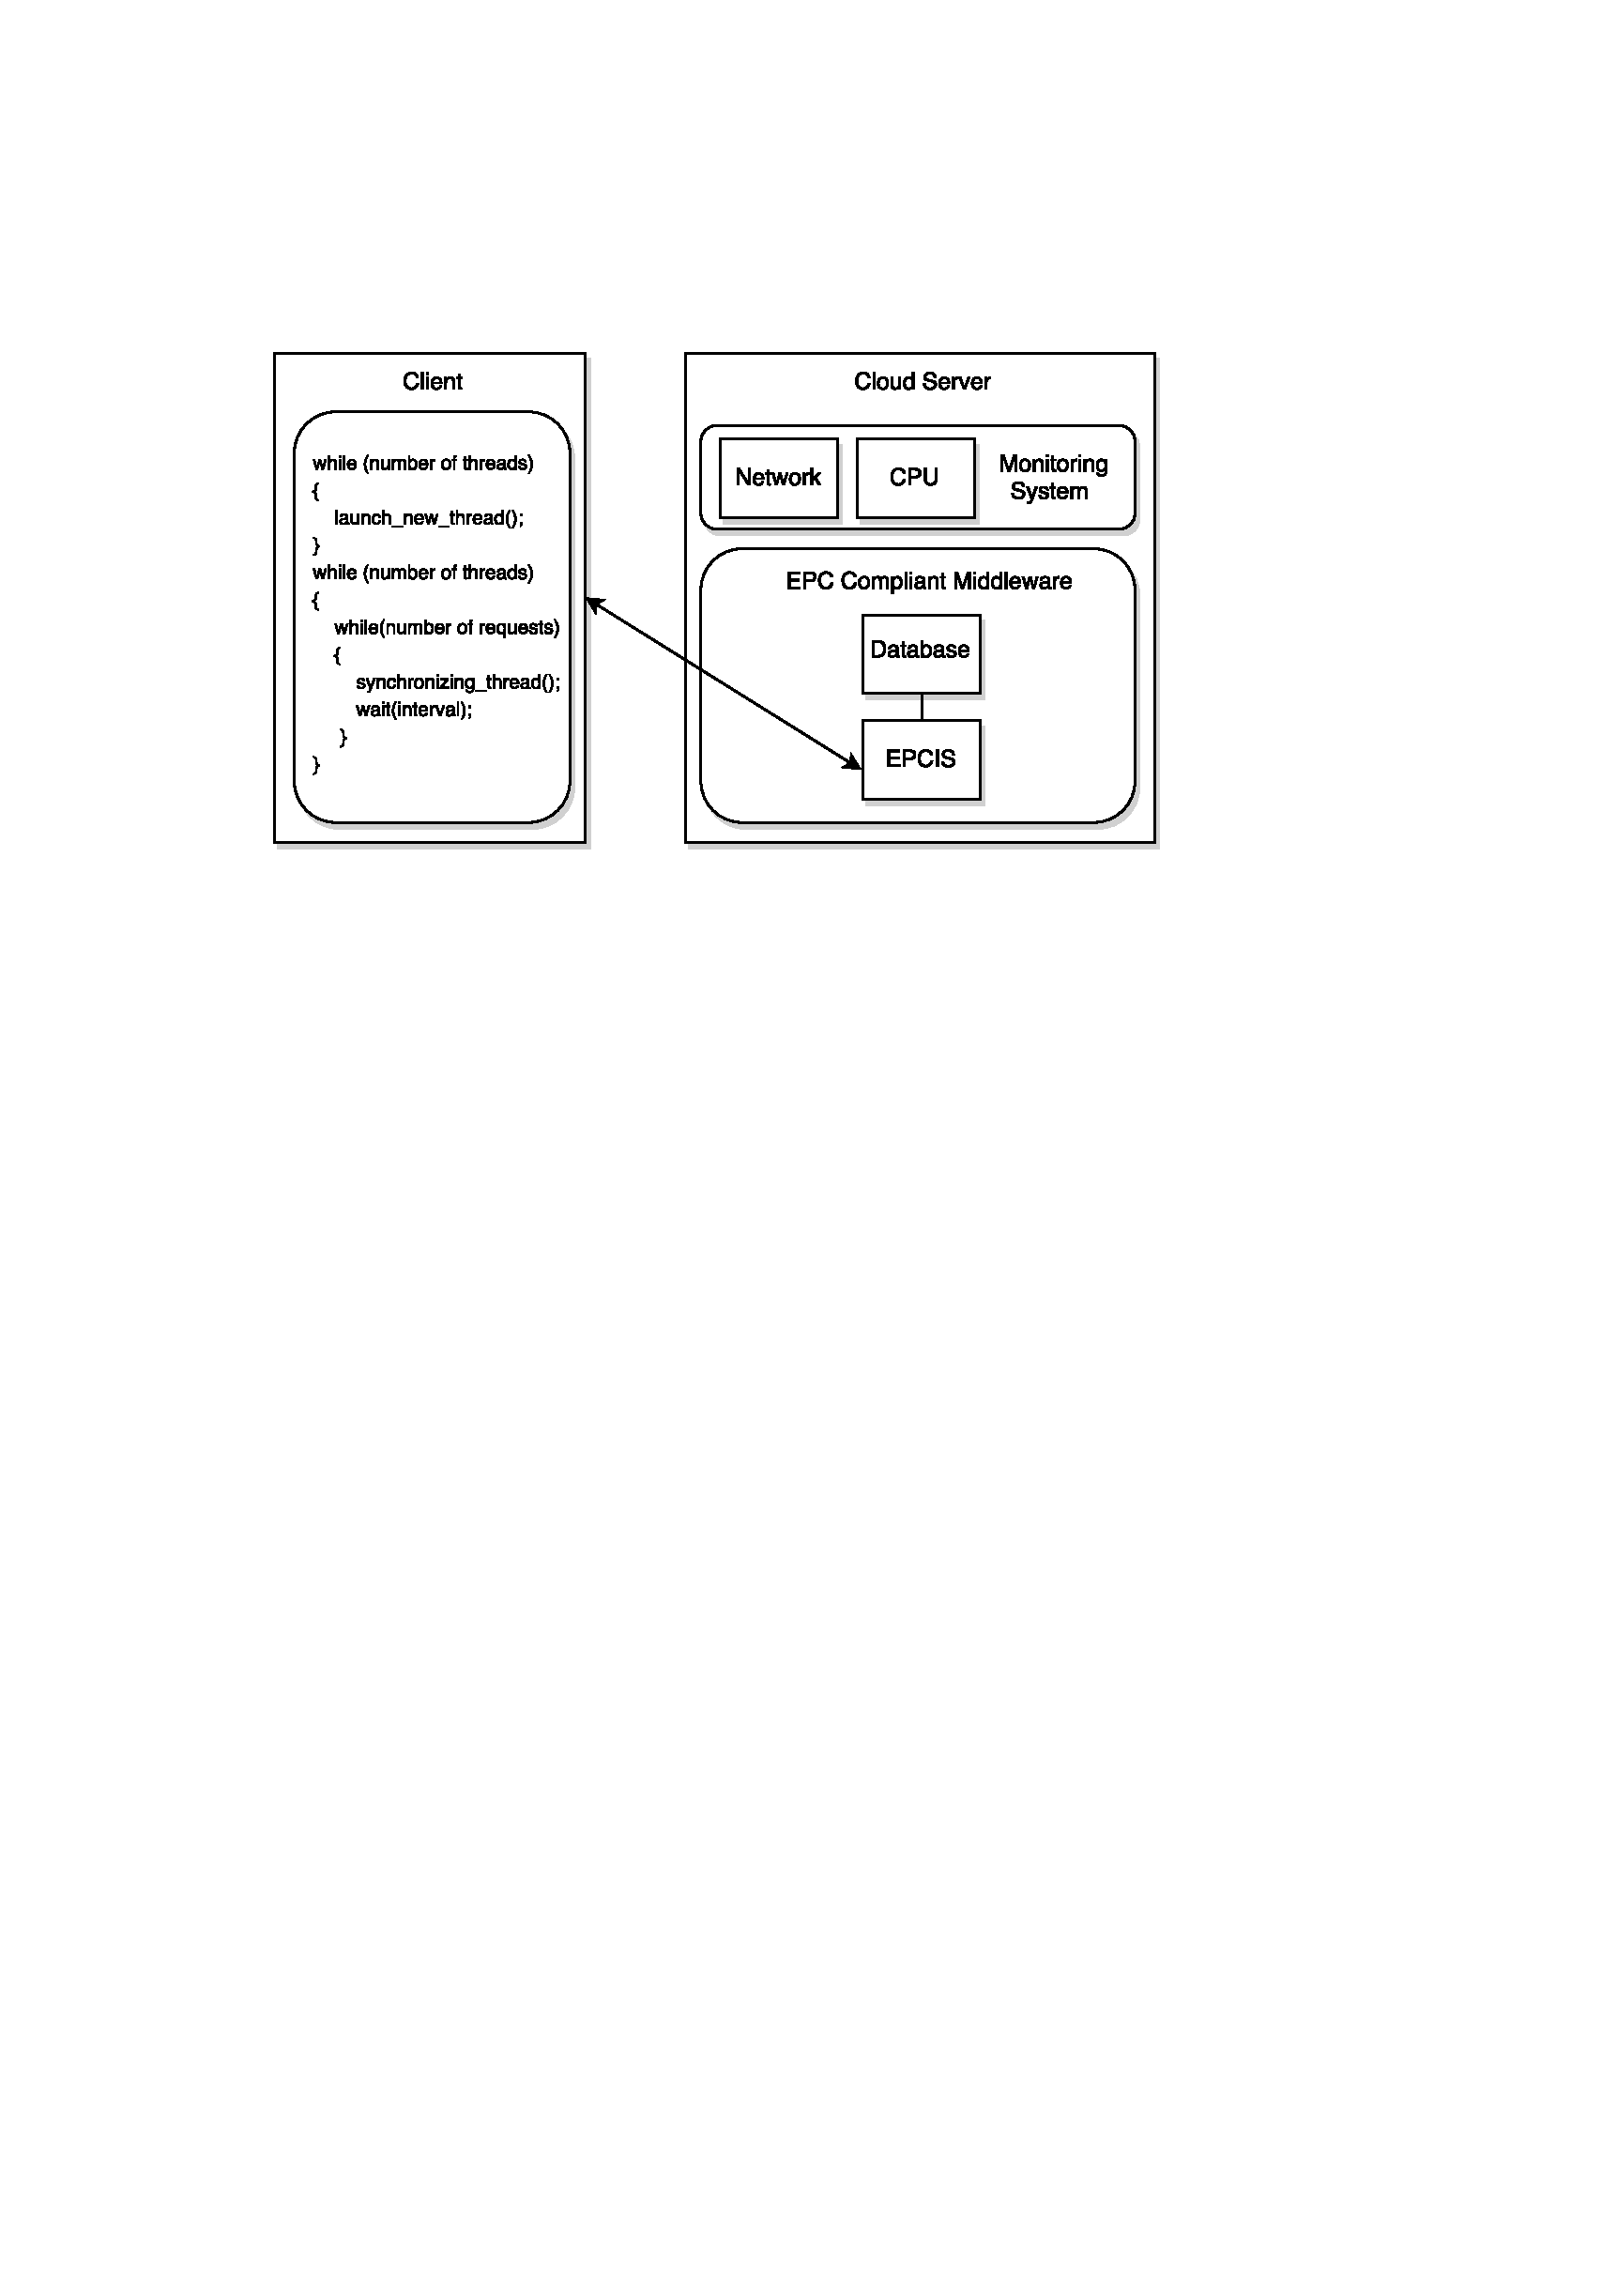
\includegraphics[width=.7\textwidth]{./images/eval_data_methodology}
  \caption{Data scalability evaluation methodology.}
  \label{fig:eval_data_methodology}
\end{figure}

The analysis of these metrics allows to observe how the performance and behavior of the \gls{EPCIS}
module is affected regarding the amount of events that are processed.

% Evaluation Methodologies : Latency
\subsection{Latency Interaction}
\label{sub:eval_methodology_latency}
To evaluate the response time between an event that occurs in the smart place and the corresponding
action that is triggered in the smart place, according the proposed methodology in Figure~\ref{fig:eval_latency_methodology}.\\

% Latency Interaction Evaluation Methodology Figure
\begin{figure}[ht!]
  \centering
  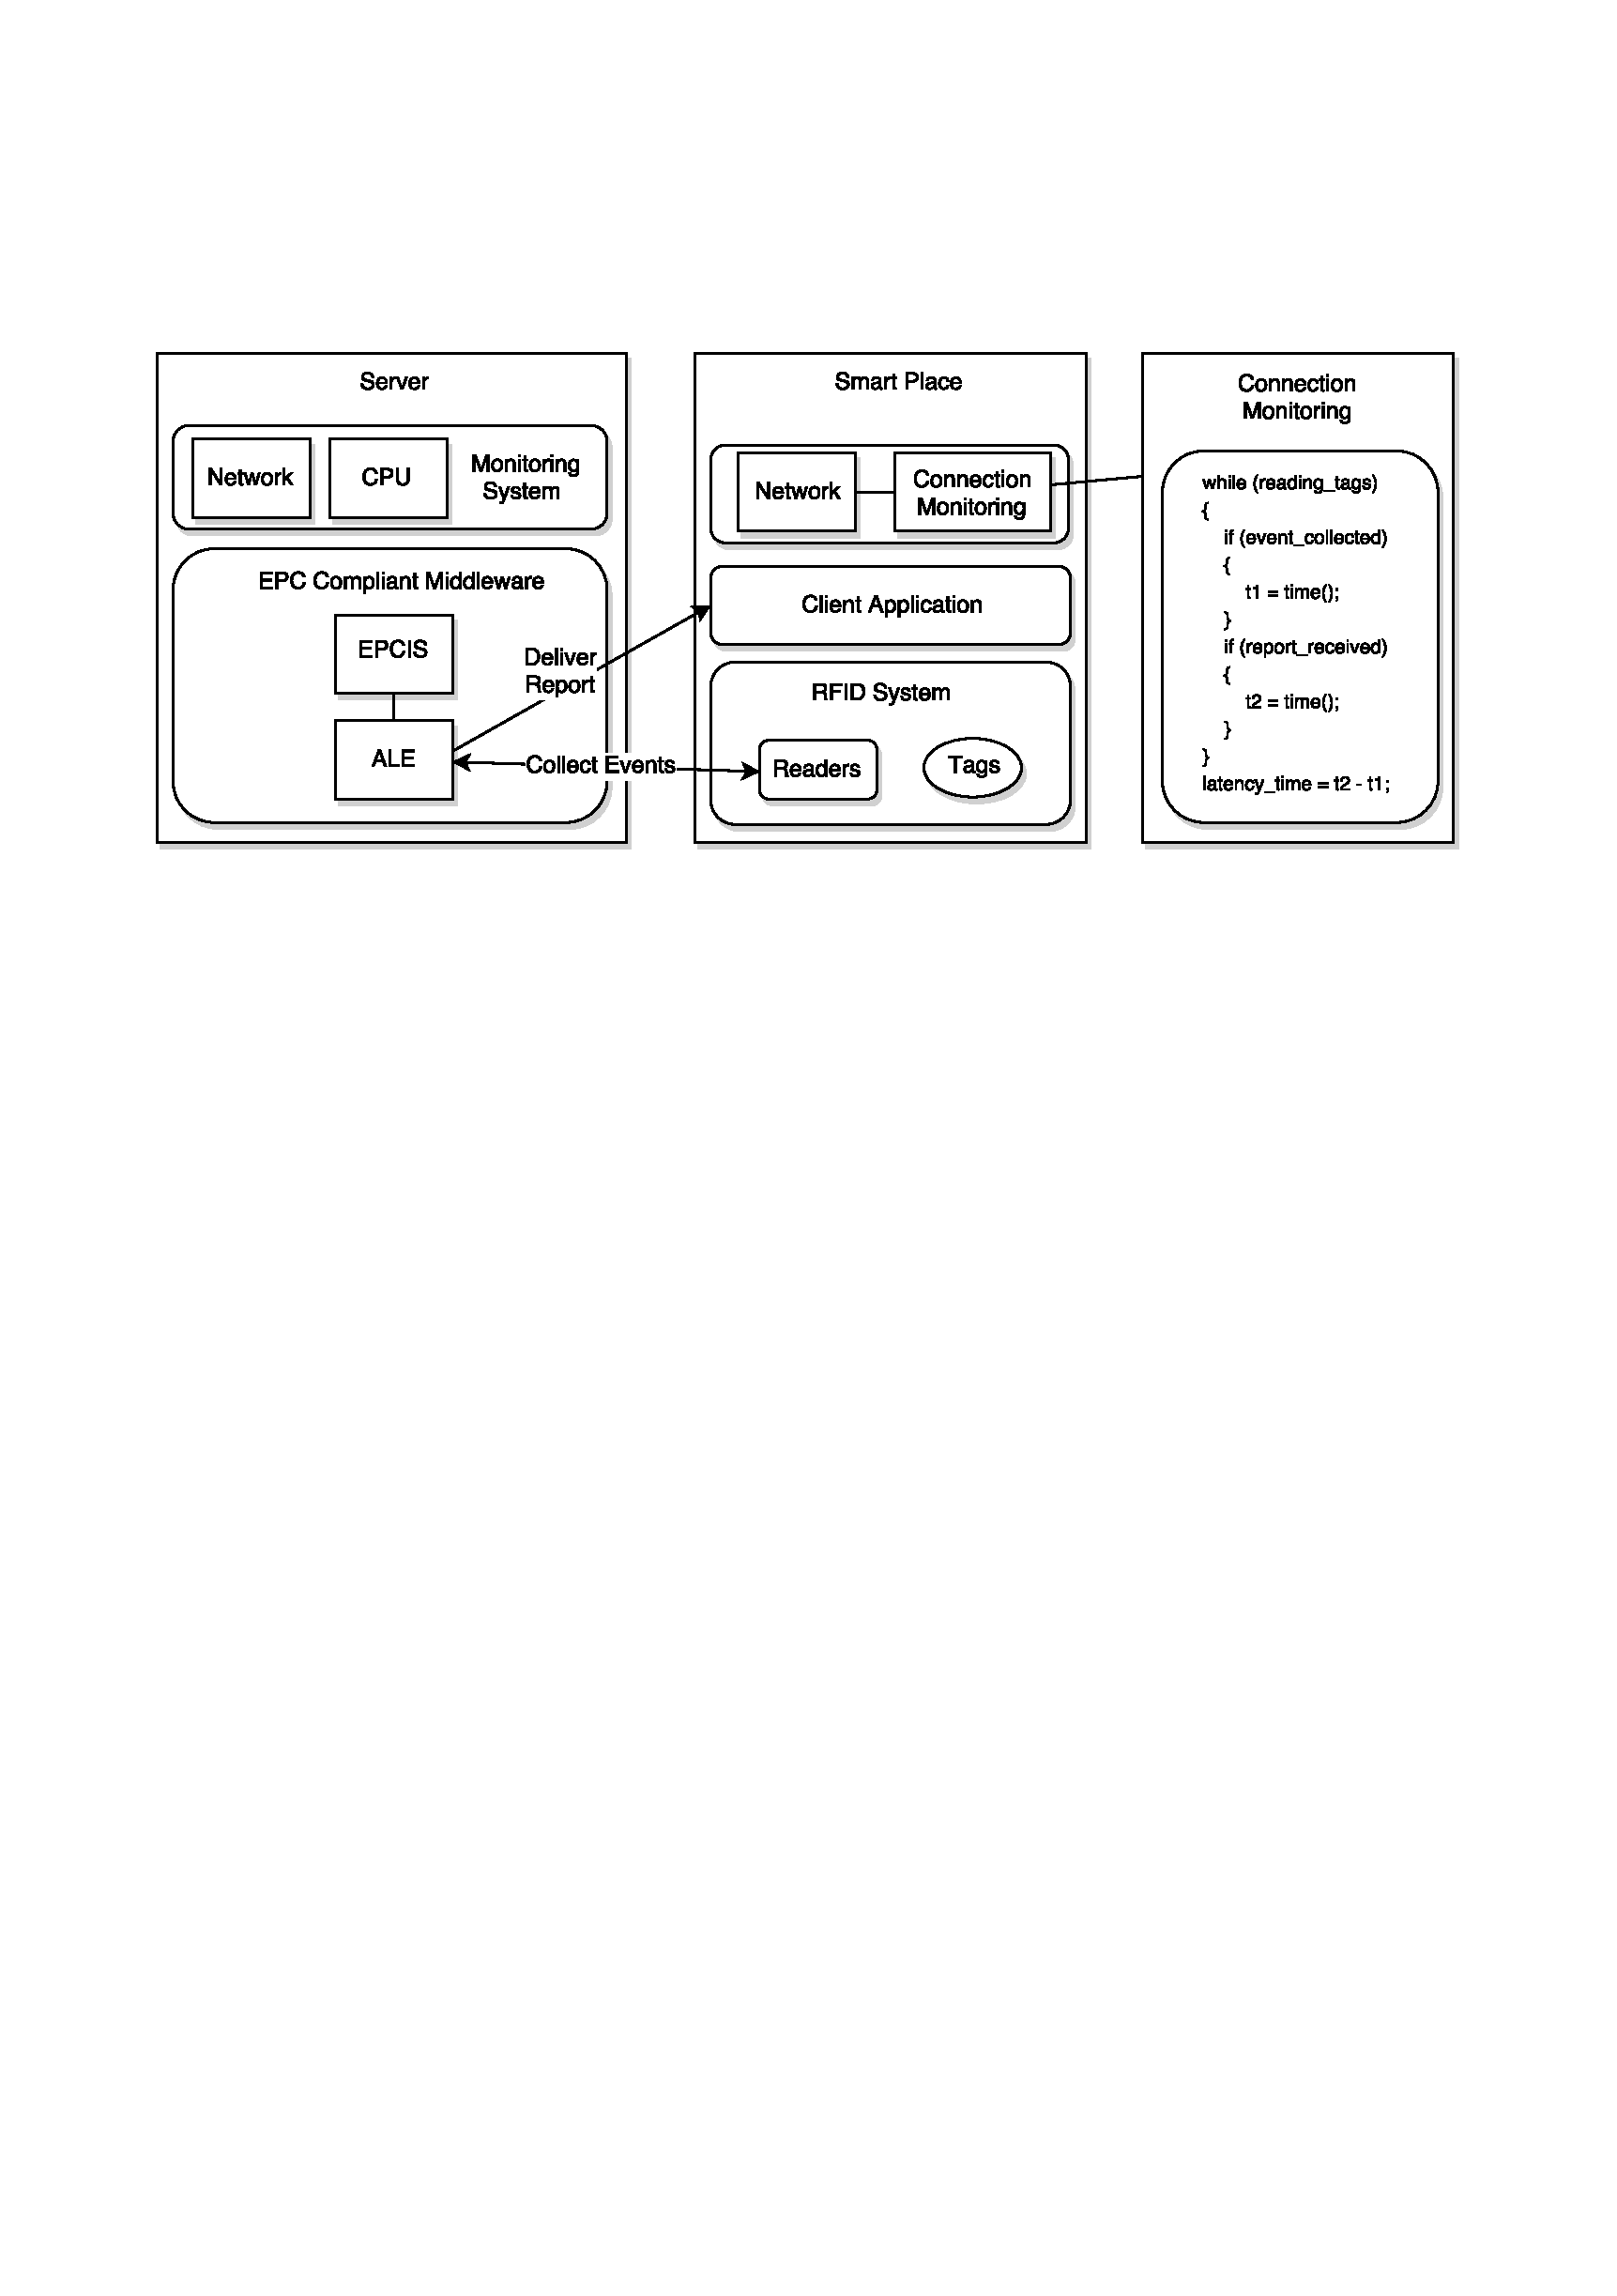
\includegraphics[width=.9\textwidth]{./images/eval_latency_methodology}
  \caption{Latency interaction evaluation methodology.}
  \label{fig:eval_latency_methodology}
\end{figure}

The \gls{ALE} module is responsible to collect and process the reader events and take the
correct decisions based on those events. In the Fosstrak implementation the collection and processing
of reader events is performed according to an \textit{Event Cycle} specification. The \textit{Event Cycle}
is a set of periodical read cycles where the \gls{ALE} module collect the events from readers. The data
about the \textit{Event Cycle} is delivered to the client through a report. The information in the report
can be used to notify the client regarding a situation in the smart place or even to trigger a new event
in the smart place such as open or close a door.\\

The smart place is running a monitoring system that stores information about the incoming and outgoing
connections. The Fosstrak \gls{ALE} module can be configured to generate information to register
when a new event is processed and also when a new reports is delivered to the client. Thus, with the
information provided by the monitoring system and the \gls{ALE} module it is possible to calculate
the latency request for an event that occurs in the smart place.\\

With this methodology we intend to obtain information regarding how the communication time is spent
when a event is triggered in the smart place the approaches described in \ref{sec:smart_place_architecture}.
In order to determine what approach is more adequate to host the application middleware, the proposed
metrics are considered:

% Metrics
\begin{itemize}
  \item \textit{Event Latency}: the time spent from the moment that an event is triggered in the
  smart place to the moment when the client application receives the notification of the event.
  \item \textit{Upload Latency}: the time spent from the moment that an event is triggered in the
  smart place from the moment when the \gls{ALE} module process the event.
  \item \textit{Processing Latency}: the time spent from the moment that the \gls{ALE} module process
  an event from the moment that the \textit{Event Cycle} report is created.
  \item \textit{Response Latency}: the time spent from the moment that the \gls{ALE} module delivers
  the \textit{Event Cycle} report to the moment that the client receives it.
\end{itemize}

The analysis of those metrics will allow us to compare the performance of both approaches and help to
determine which one is more adequate to host \gls{RFID} applications middleware.

% Evaluation Setup
\section{Evaluation Setup}
\label{sec:eval_setup}
To perform the evaluation experiments we choose \gls{AWS} as cloud provider. All the experiments were
conducted in \gls{AWS} \gls{EC2} instances running the Amazon Linux AMI operating system. The virtual
machines presents a configuration with a 2.5\textit{\gls{GHz}} single-core processor with 1\textit{\gls{GB}} of
\gls{RAM}. In the fog-aprroach configuration, where the \gls{ALE} module is provisioned in the smart place,
the experiments were conducted in a virtual machine with a 2.6\textit{\gls{GHz}} dual-core processor
with 2\textit{\gls{GB}} of \gls{RAM} and running the \textit{Linux Ubuntu 14.04.1 LTS} operating system.
Regarding the smart place infrastructure, the evaluation was performed through a \gls{ADSL} connection
and the Rifidi Emulator\footnote{http://rifidi.org} was used to emulate the physical readers that are
in the smart place.\\

Regarding software components, the application stack is composed of the \textit{Apache Tomcat 7.0.52.0}\footnote{http://tomcat.apache.org/}
with \textit{Java} version \textit{1.7.0} update \textit{79}. The \gls{RFID} middleware used was the Fosstrak
described in section \ref{sub:fosstrak}. The middleware stack is available at the Fosstrak's\footnote{http://fosstrak.github.io/}
source control system, and the versions were: a) \textit{FCServer} version \textit{1.2.0}; b) \textit{Capture Application}
version \textit{0.1.1}; and c) \textit{\gls{EPCIS} Repository} version \textit{0.5.0}. Furthermore,
the \gls{EPCIS} Repository was connected to a \textit{MySQL server} version \textit{5.5} that stores
all the \gls{EPCIS} events.

% Performed Experiments
\section{Experiments Performed}
\label{sec:eval_experiments}
The experiments performed in our evaluation were based on the scenario and data from the RFIDToys\cite{Correia:Thesis:2014}
Master Thesis.

\subsection{Data Scalability}
\label{sub:eval_exp_data}
To evaluate the data scalability for the Fosstrak middleware we use the data recorded with the Rec\&Play
- which is able to record \gls{RFID} sessions that stores the events occurred in the smart place
maintaining the order and time from the beginning of the session - module were used as base to execute
the tests.\\

As described in Section \ref{sub:eval_methodology_data}, the methodology consists in simulate a given
number of readers that are in the warehouse. The simulation was performed through Jmeter\footnote{http://jmeter.apache.org/},
a Java application designed to perform load testing and measure the application performance.
In order to reproduce some situations that can occur in a real smart place, we perform the following
variations in the tests:

% Test variations
\begin{itemize}
  \item\textbf{Standard} The test is executed with the amount of events and period from the recorded session.
  \item\textbf{Double of Requests} The test is executed with the period and twice of events from the recorded
  session.
  \item\textbf{Half of Interval} The test is executed with the amount of events and half of the period from
  the recorded session.
\end{itemize}

Each test case was executed simulating 5 readers at most in two scenarios, \textbf{Baseline} and
\textbf{Track 3 Laps}.

\subparagraph{Baseline}
\label{subp:eval_exp_data_baseline}
In the \textbf{Baseline} scenario the session contains the data recorded based in the events generated
during a 1 lap in the track. The parameters used to execute the test for this scenario are described in
Table~\ref{tab:baseline_parameters}.

% Baseline parameters
\begin{table}[ht!]
  \begin{tabular}{|c|c|}
    \hline
    Number of Events & Period \\ \hline
    1593             & 82ms   \\ \hline
  \end{tabular}
  \caption{Baseline evaluation parameters.}
  \label{tab:baseline_parameters}
\end{table}

% Baseline results
\begin{figure}[ht!]
\centering
\begin{subfigure}{.5\textwidth}
  \centering
  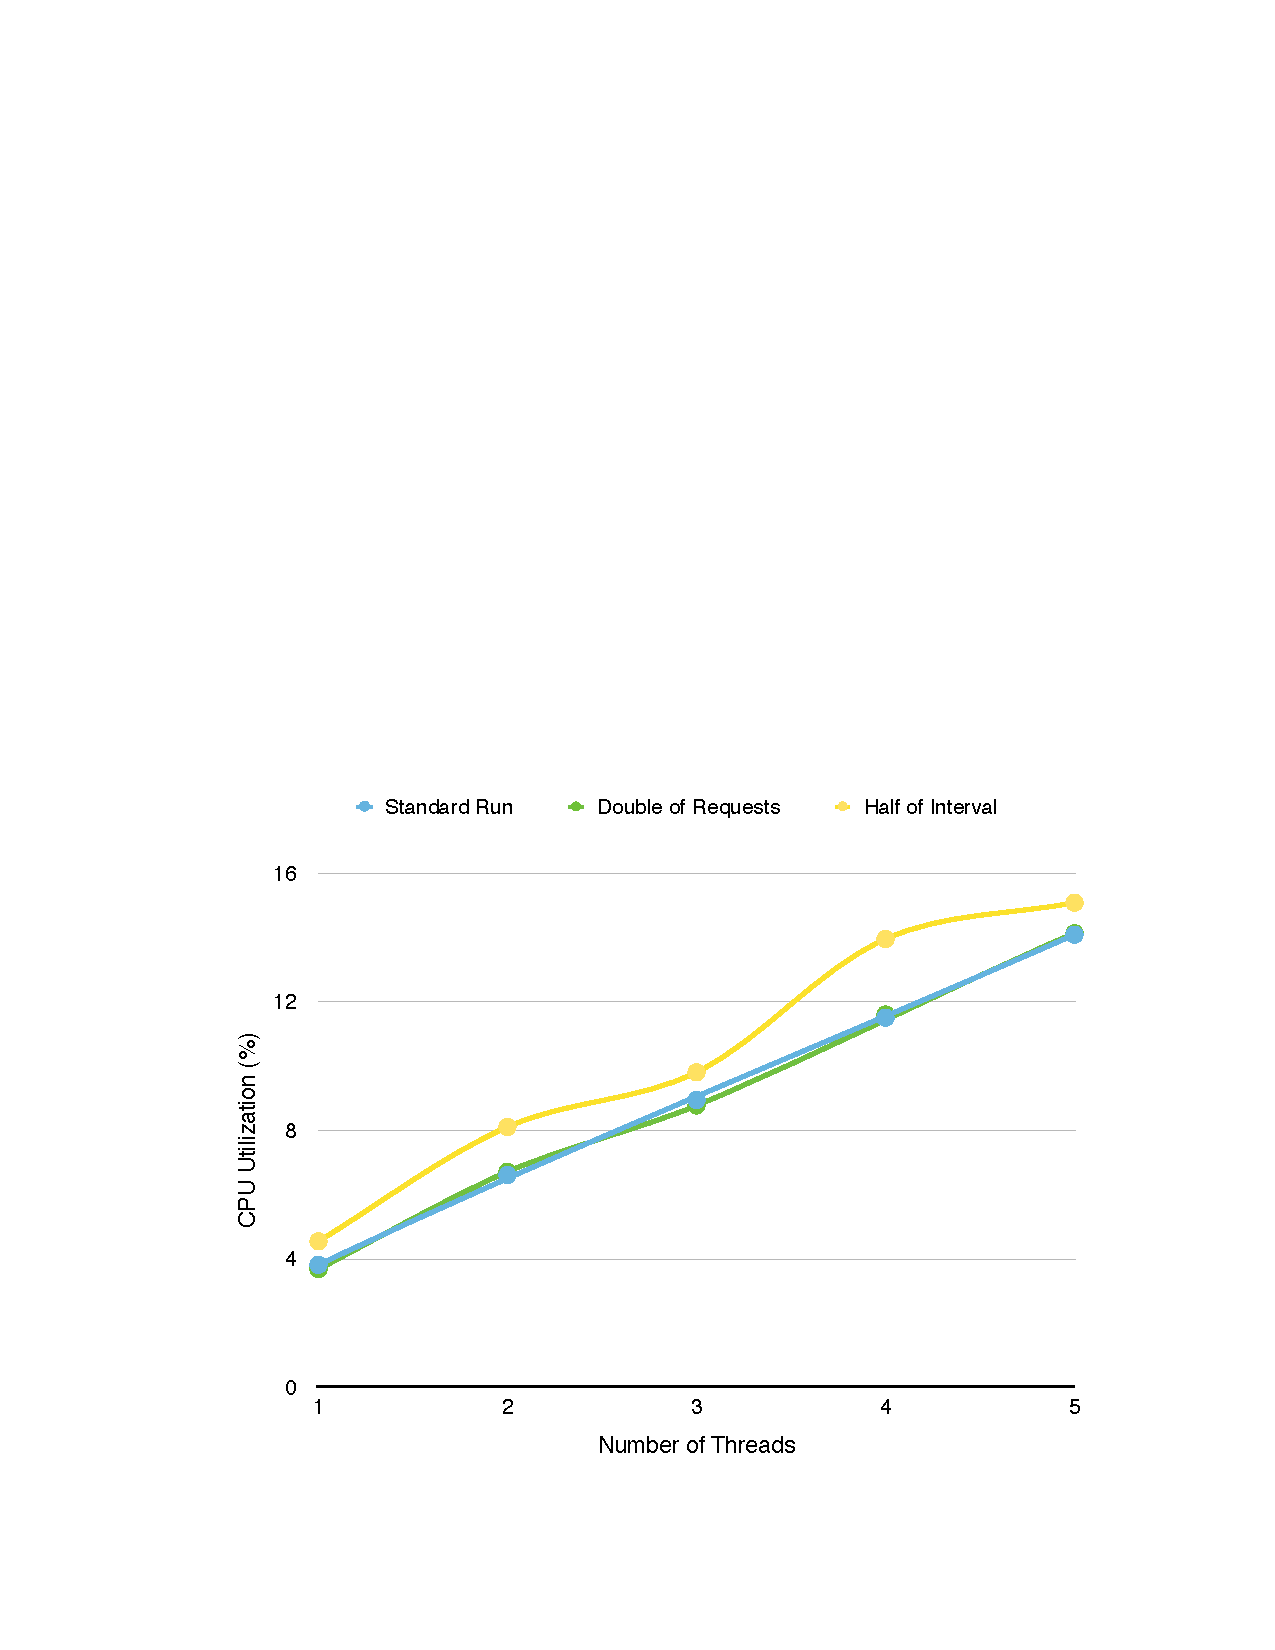
\includegraphics[width=\linewidth]{./images/cpu_1_lap}
  \caption{Baseline CPU Utilization.}
  \label{fig:eval_baseline_cpu}
\end{subfigure}%
\begin{subfigure}{.5\textwidth}
  \centering
  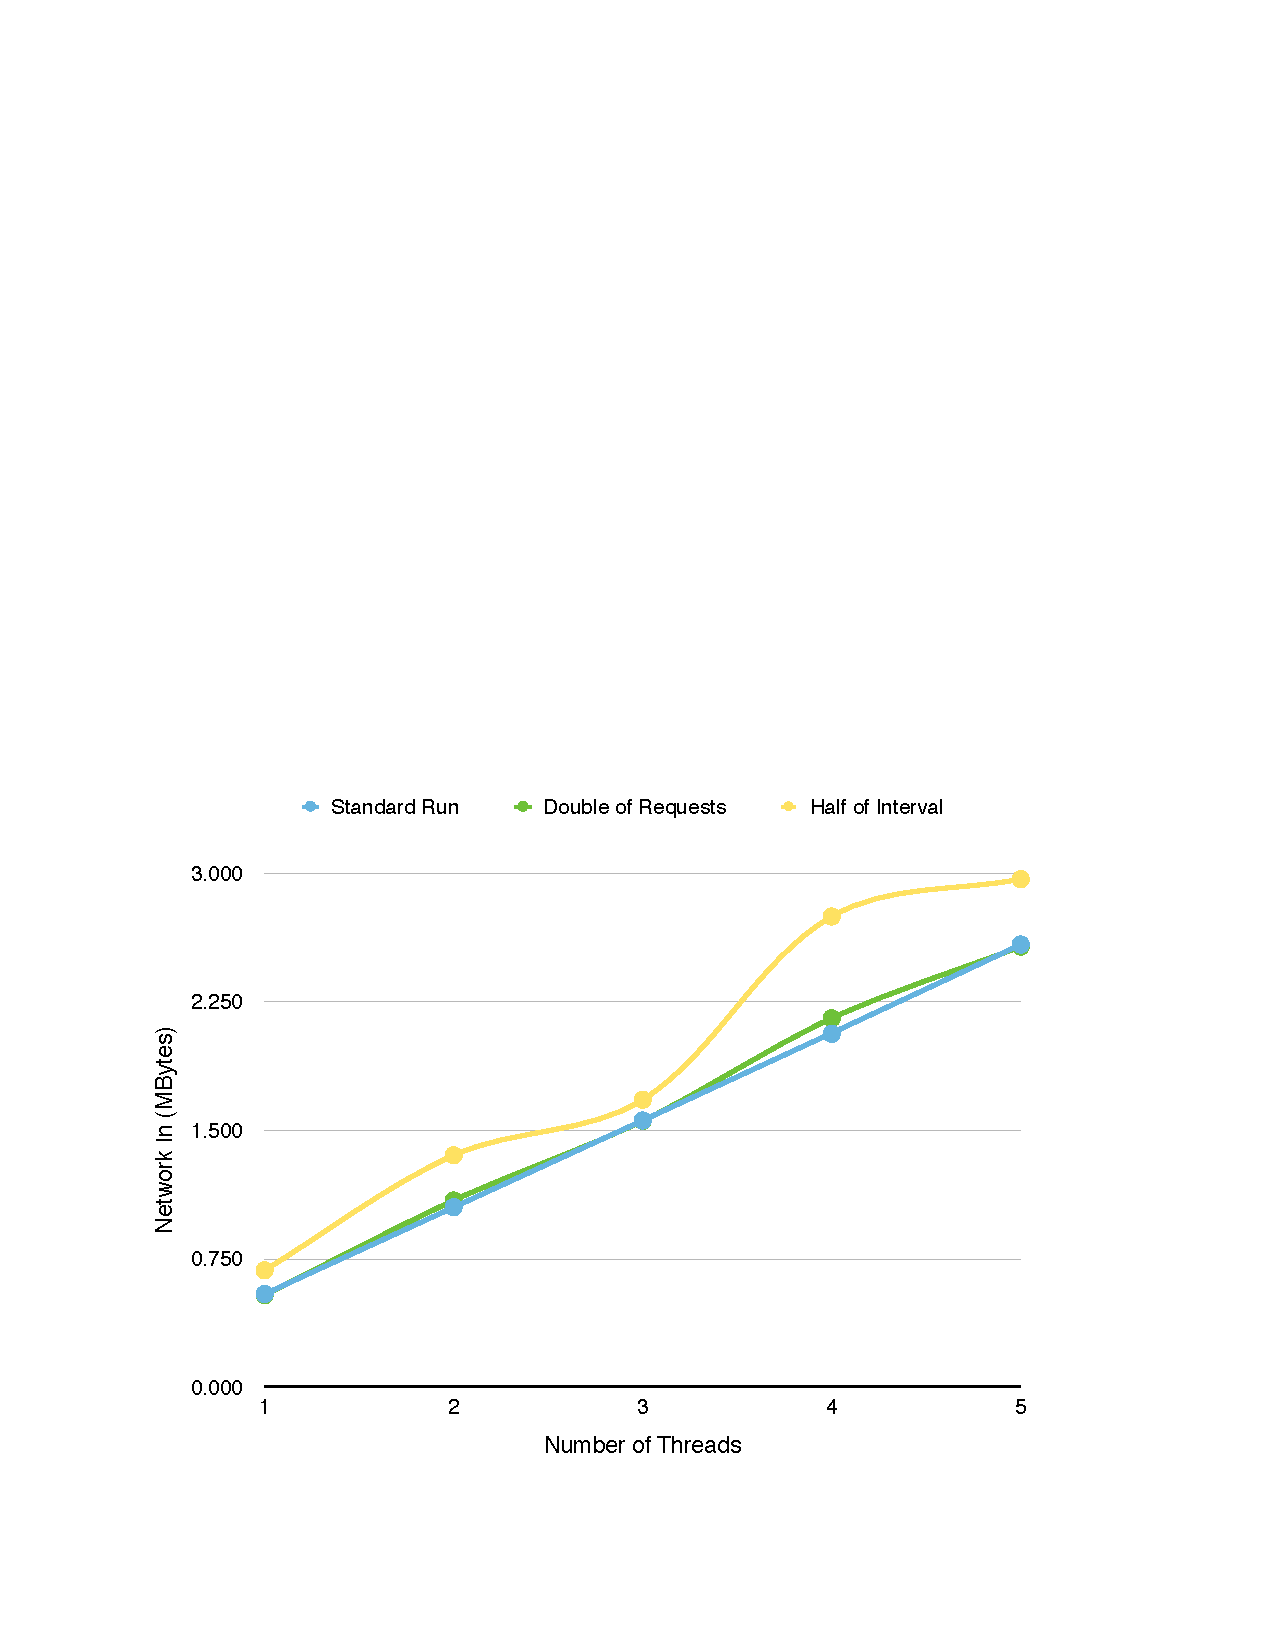
\includegraphics[width=\linewidth]{./images/network_1_lap}
  \caption{Baseline Network traffic.}
  \label{fig:eval_baseline_network}
\end{subfigure}
\caption{Baseline performance results.}
\label{fig:eval_baseline_results}
\end{figure}

Figure~\ref{fig:eval_baseline_cpu} presents the system metric \textit{CPU Utilization} for the current
experiment. Comparing the values obtained in the experiment for the three variations, for the
\textit{Standard} and the \textit{Double of Requests} variations the behavior is very similar and tend
to take a linear pattern. For the \textit{Half of Interval} variation, it is possible to observe
that in this variation, the metric value is always higher - maximum close to 16$\%$ - compared with the other
variations. The metric behavior changes according the number of threads that are sending events and
tend to take a sinusoidal pattern.\\

The system metric \textit{Network In}, presented in Figure~\ref{fig:eval_baseline_network}, assumes a
similar behavior to the previous metric. For the \textit{Standard} and \textit{Double of Requests} variations,
the values are similar and the behavior tend to take a linear pattern. It is possible to take the same
conclusions for the \textit{Half of Interval} variation, where the values are always higher - maximum
close to 3 \gls{MB} - and the behavior tends to take a sinusoidal pattern.

\subparagraph{Track 3 Laps}
\label{subp:eval_exp_data_3laps}
In the \textbf{Track 3 Laps} scenario the session contains the data recorded based in the events generated
during 3 laps in the track. The parameters used to execute the test for this scenario are described in
Table~\ref{tab:3laps_parameters}.\\

% 3 Lap parameters
\begin{table}[ht!]
  \begin{tabular}{|c|c|}
    \hline
    Number of Events & Period \\ \hline
    8895             & 57ms   \\ \hline
  \end{tabular}
  \caption{3 Lap evaluation parameters.}
  \label{tab:3laps_parameters}
\end{table}

% 3 Lap results
\begin{figure}[ht!]
\centering
\begin{subfigure}{.5\textwidth}
  \centering
  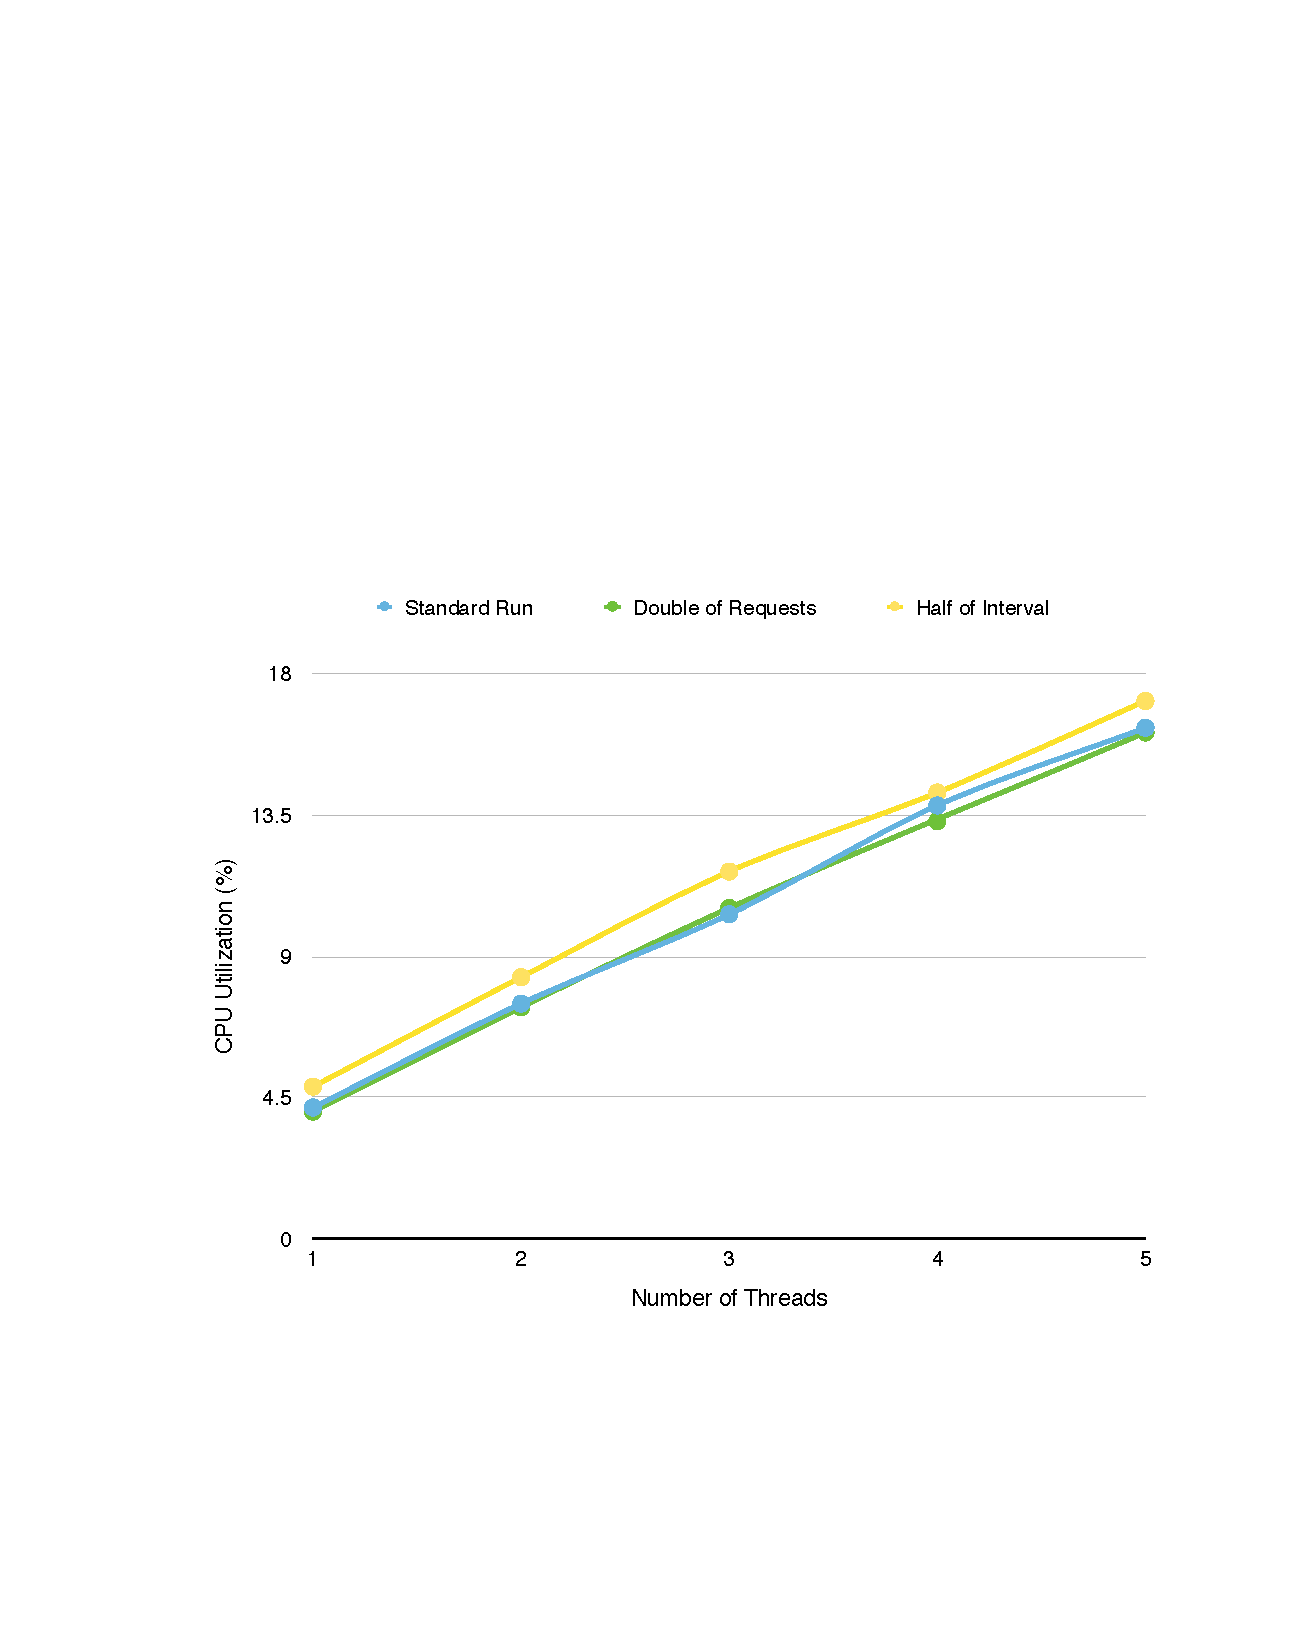
\includegraphics[width=\linewidth]{./images/cpu_3_lap}
  \caption{Track 3 Laps CPU Utilization.}
  \label{fig:eval_3laps_cpu}
\end{subfigure}%
\begin{subfigure}{.5\textwidth}
  \centering
  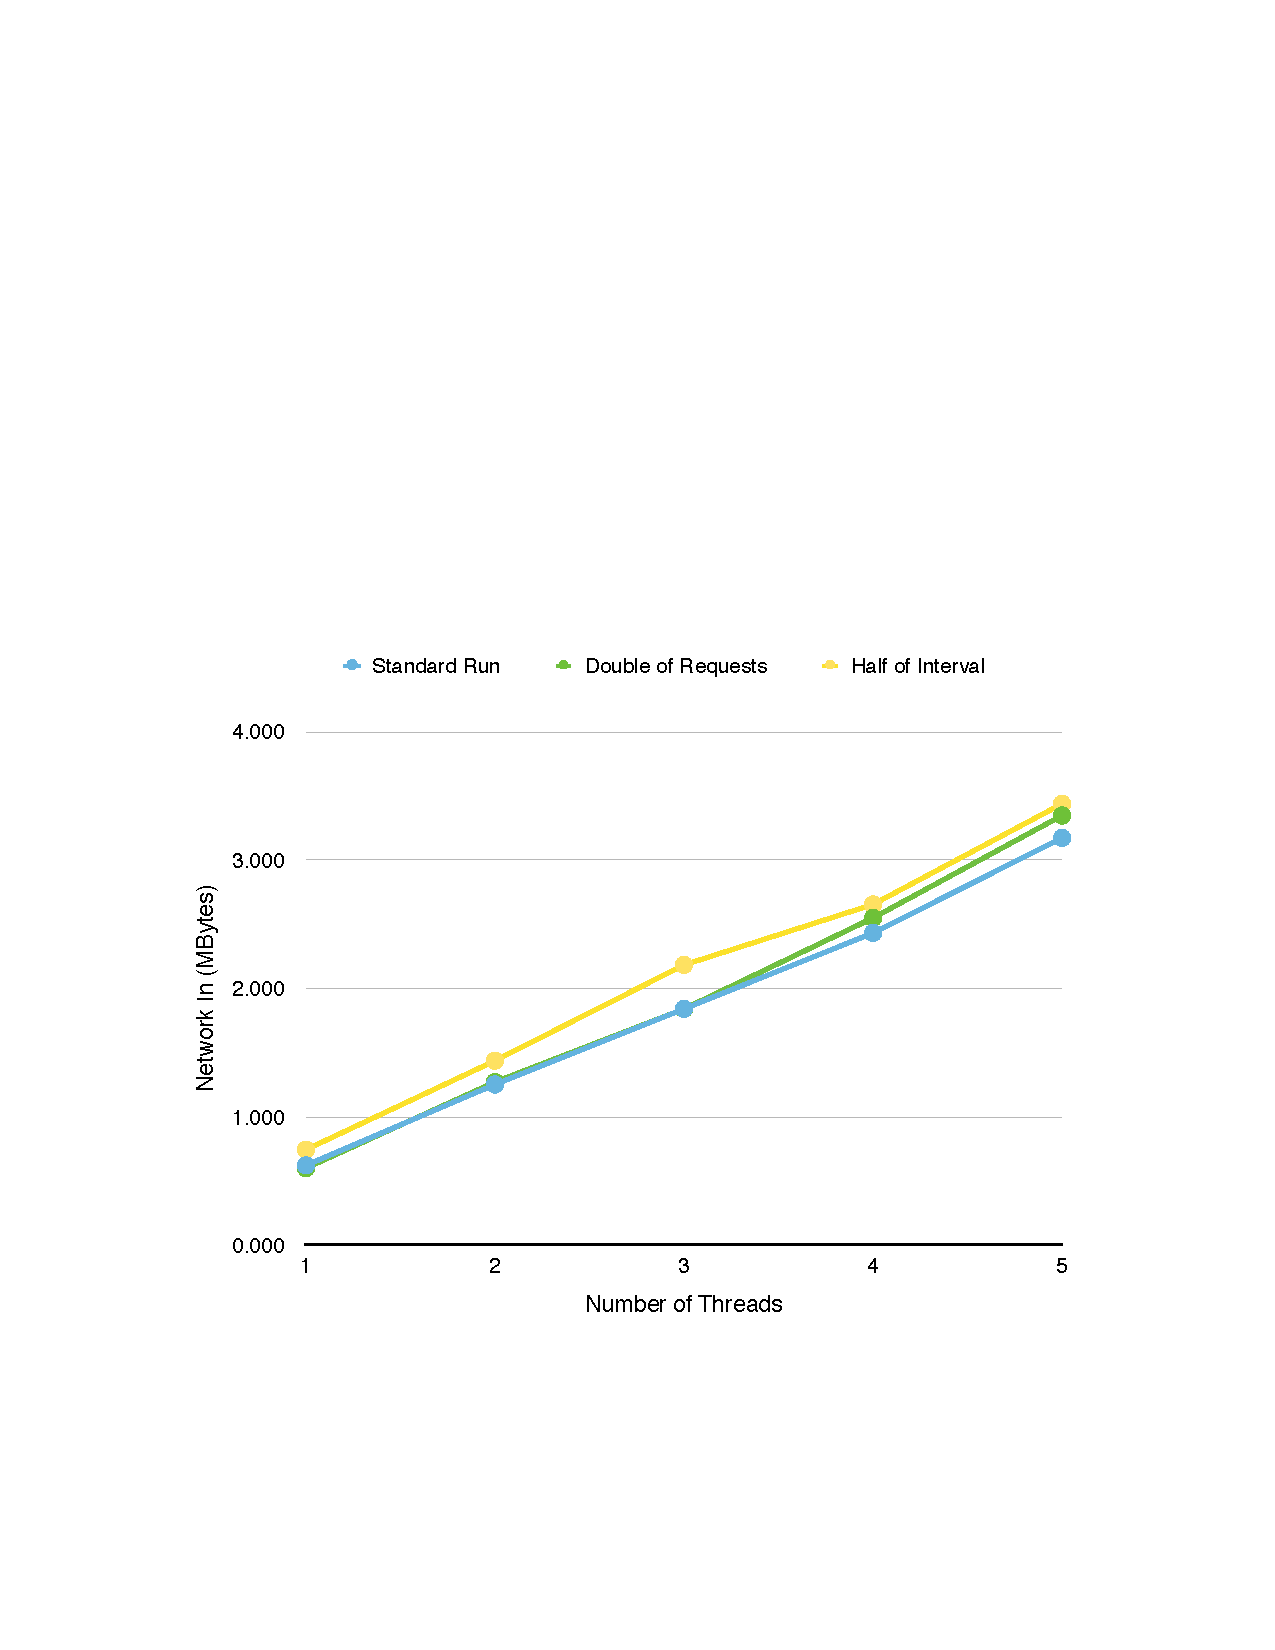
\includegraphics[width=\linewidth]{./images/network_3_lap}
  \caption{Track 3 Laps Network traffic.}
  \label{fig:eval_3laps_network}
\end{subfigure}
\caption{Track 3 Lap performance results.}
\label{fig:eval_3laps_results}
\end{figure}

Figure~\ref{fig:eval_3laps_cpu} presents the system metric \textit{CPU Utilization} for the current
experiment. Comparing the values values obtained in the experiment, it is possible to observe that
the values are very similar for all variations. The \textit{Half of Interval} continues to present
the highest values - maximum close to 18$\%$ - while the other variations presents almost identical
values. Regarding the metric behavior, all variations tends to take a linear pattern.\\

As in the previous experiment, the system metric \textit{Network In}, presented in Figure~\ref{fig:eval_3laps_network},
is very similar to the previous regarding its values and behavior. The \textit{Half of Interval}
variation still presents the highest values - maximum close to 3.5 \gls{MB} - but as the number of
threads increase, it is possible to observe that the values of the \textit{Double of Requests}
variation tend to be close to the \textit{Half of Interval} variation.


\subsection{Latency Interaction}
\label{sub:eval_exp_latency}
To evaluate the latency interaction for an event that occurs in the smart place and the corresponding
action that is triggered in the smart place, we use the scenario where a tagged robot was programmed to
execute a given number of laps in the warehouse plant where \gls{RFID} readers are placed to detect
when the robot is approaching. During the lap the robot stops during 5 seconds near to a reader and
then continues its lap.\\

According the methodology described in Section~\ref{sub:eval_methodology_latency}, the smart place
network connection was monitored to allow the inspection of incoming and outgoing connections and
determine how the connection time is spent in the cloud-based approach and the fog-based approach,
based on the proposed metrics. In our simulation the smart place was monitored through the
\textit{tcpdump}\footnote{http://www.tcpdump.org/} tool, that allows to monitoring the packets that
are being transmitted or received over a network.\\

The simulation was performed according two different specifications for the \gls{ALE} module,
\textit{Base Event Cycle} and \textit{Half-period Event Cycle} .

% Standard Event Cycle
\subparagraph{Baseline Event Cycle}
\label{subp:eval_exp_latency_ecspec}
 In the baseline scenario, we define the \textit{Base ECspec} to configure the \gls{ALE} module. The
 configuration parameters are described in Table~\ref{table:ecspec_base}.

% Base ECspec parameters
 \begin{table}[ht!]
   \begin{tabular}{|c|c|}
     \hline
     Period & Duration \\ \hline
     10s    & 9.5s     \\ \hline
  \end{tabular}
  \caption{Base ECspec parameters.}
  \label{table:ecspec_base}
 \end{table}

\begin{figure}[ht!]
  % ECSpec local breakdown figure
  \centering
  \begin{subfigure}{.5\textwidth}
    \centering
    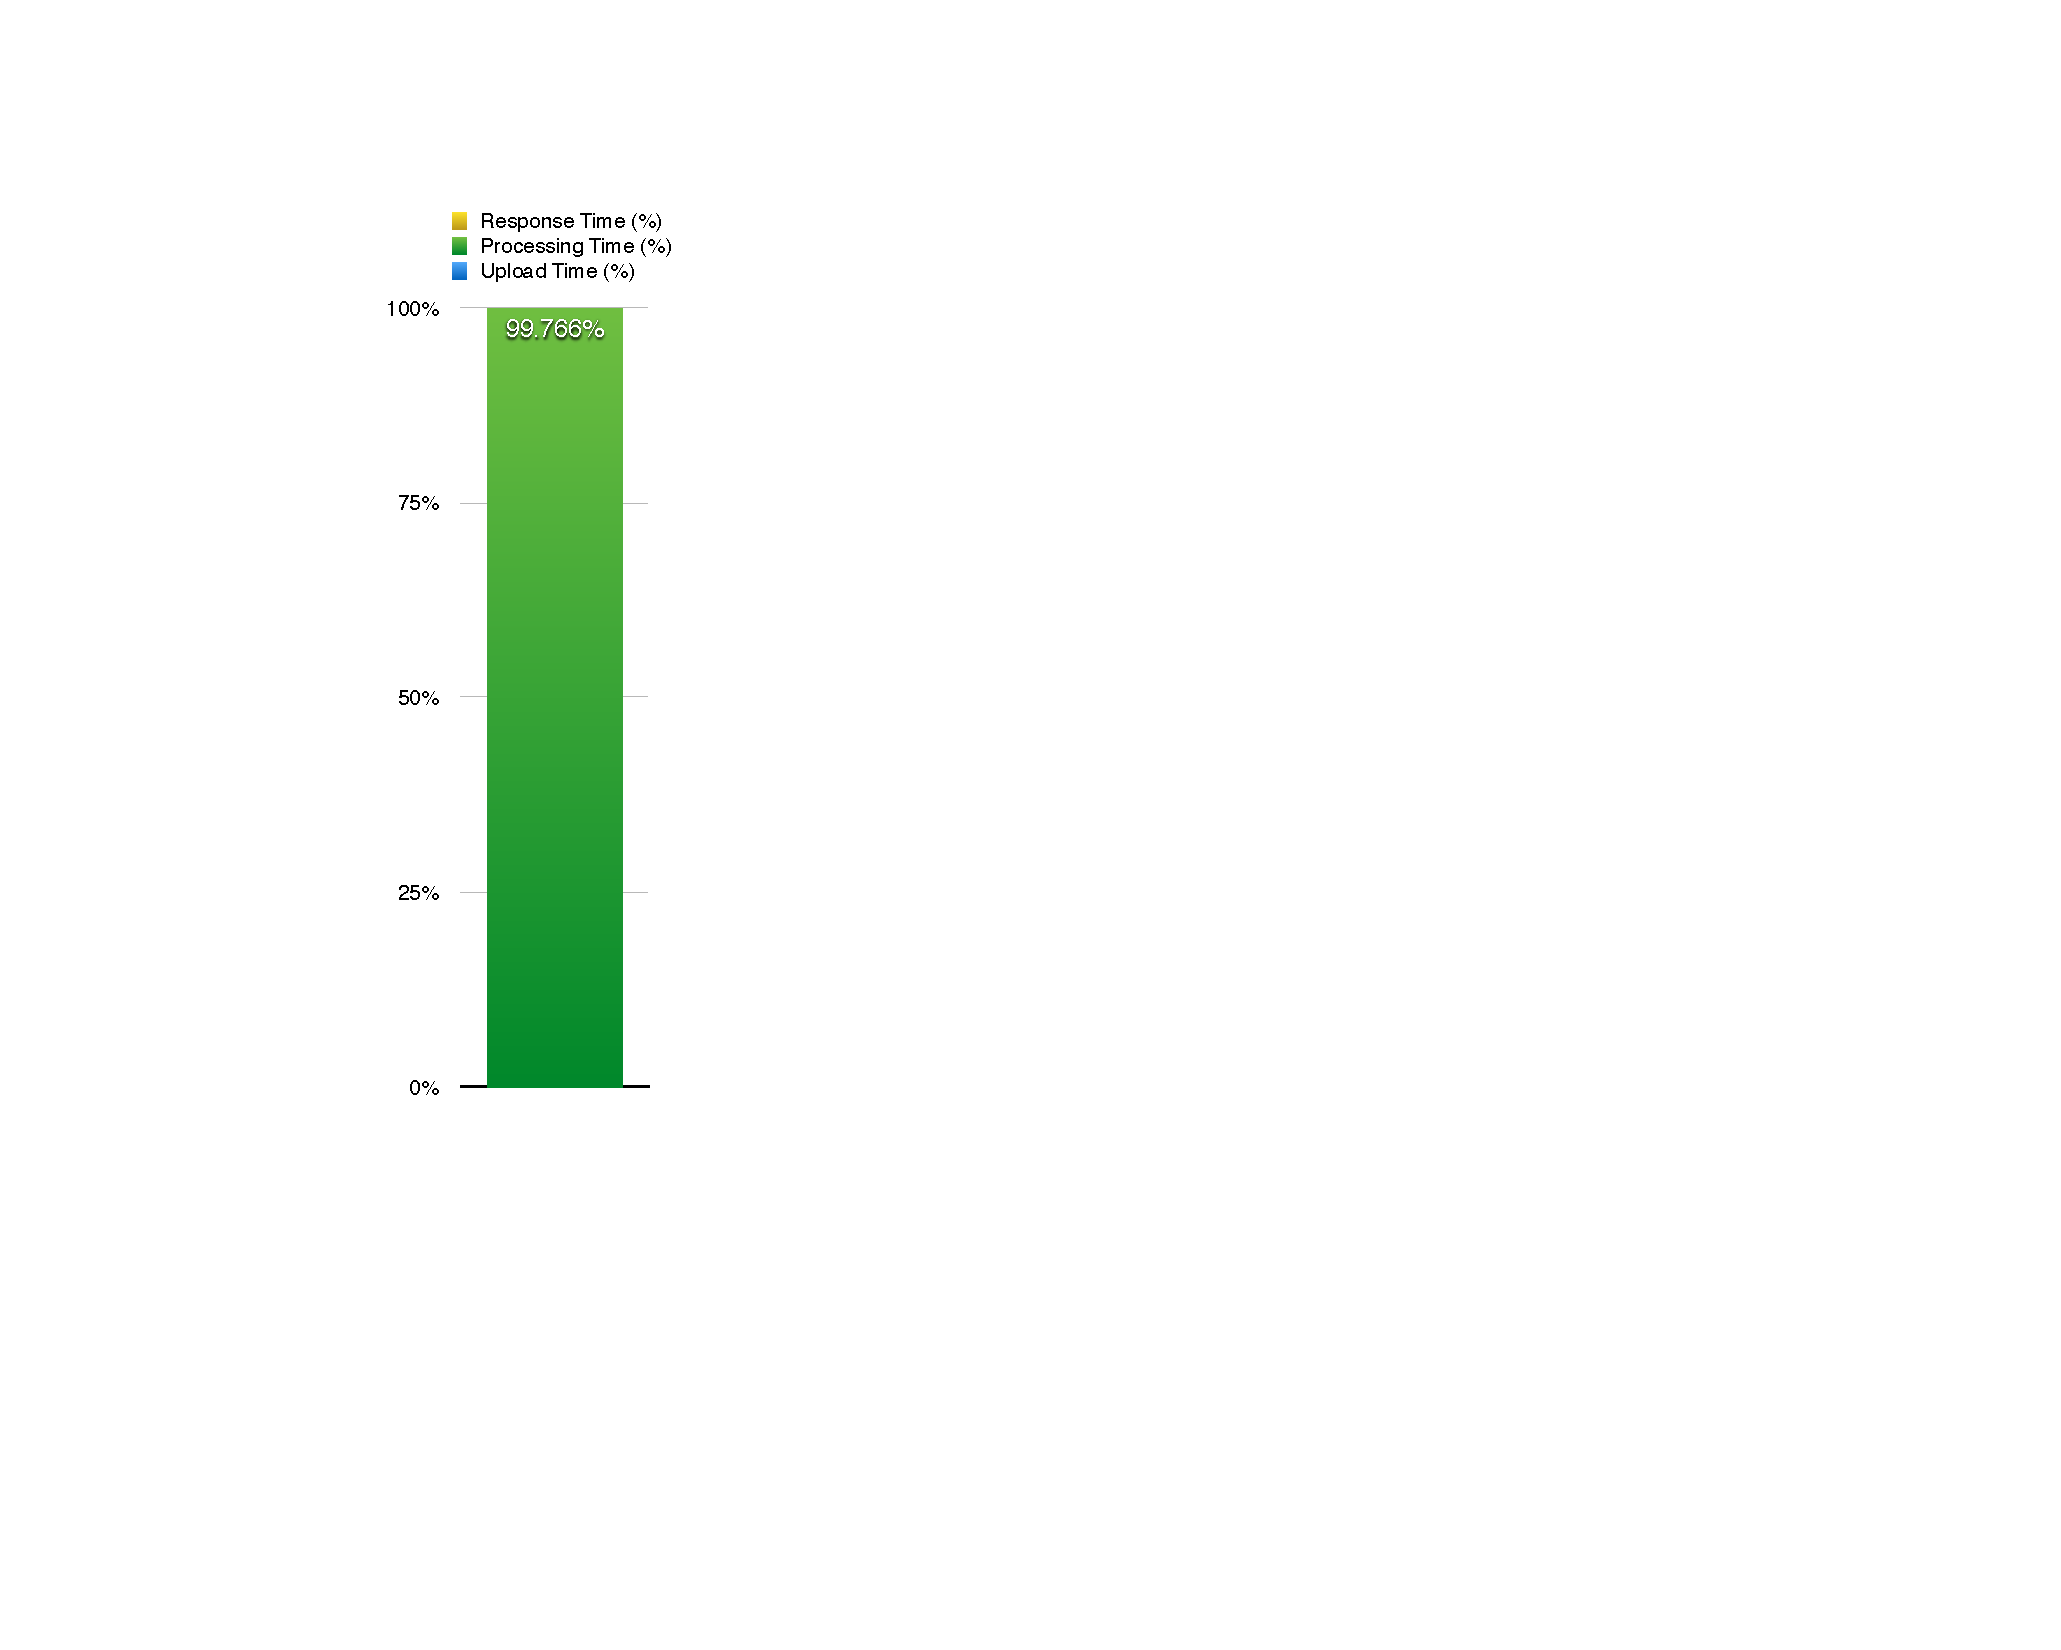
\includegraphics[width=.365\linewidth]{./images/ecspec_local_breakdown}
    \caption{Fog-based approach: baseline\\Event Cycle latency breakdown.}
    \label{fig:ecspec_local}
  \end{subfigure}%
  % ECSpec cloud breakdown figure
  \begin{subfigure}{.5\textwidth}
    \centering
    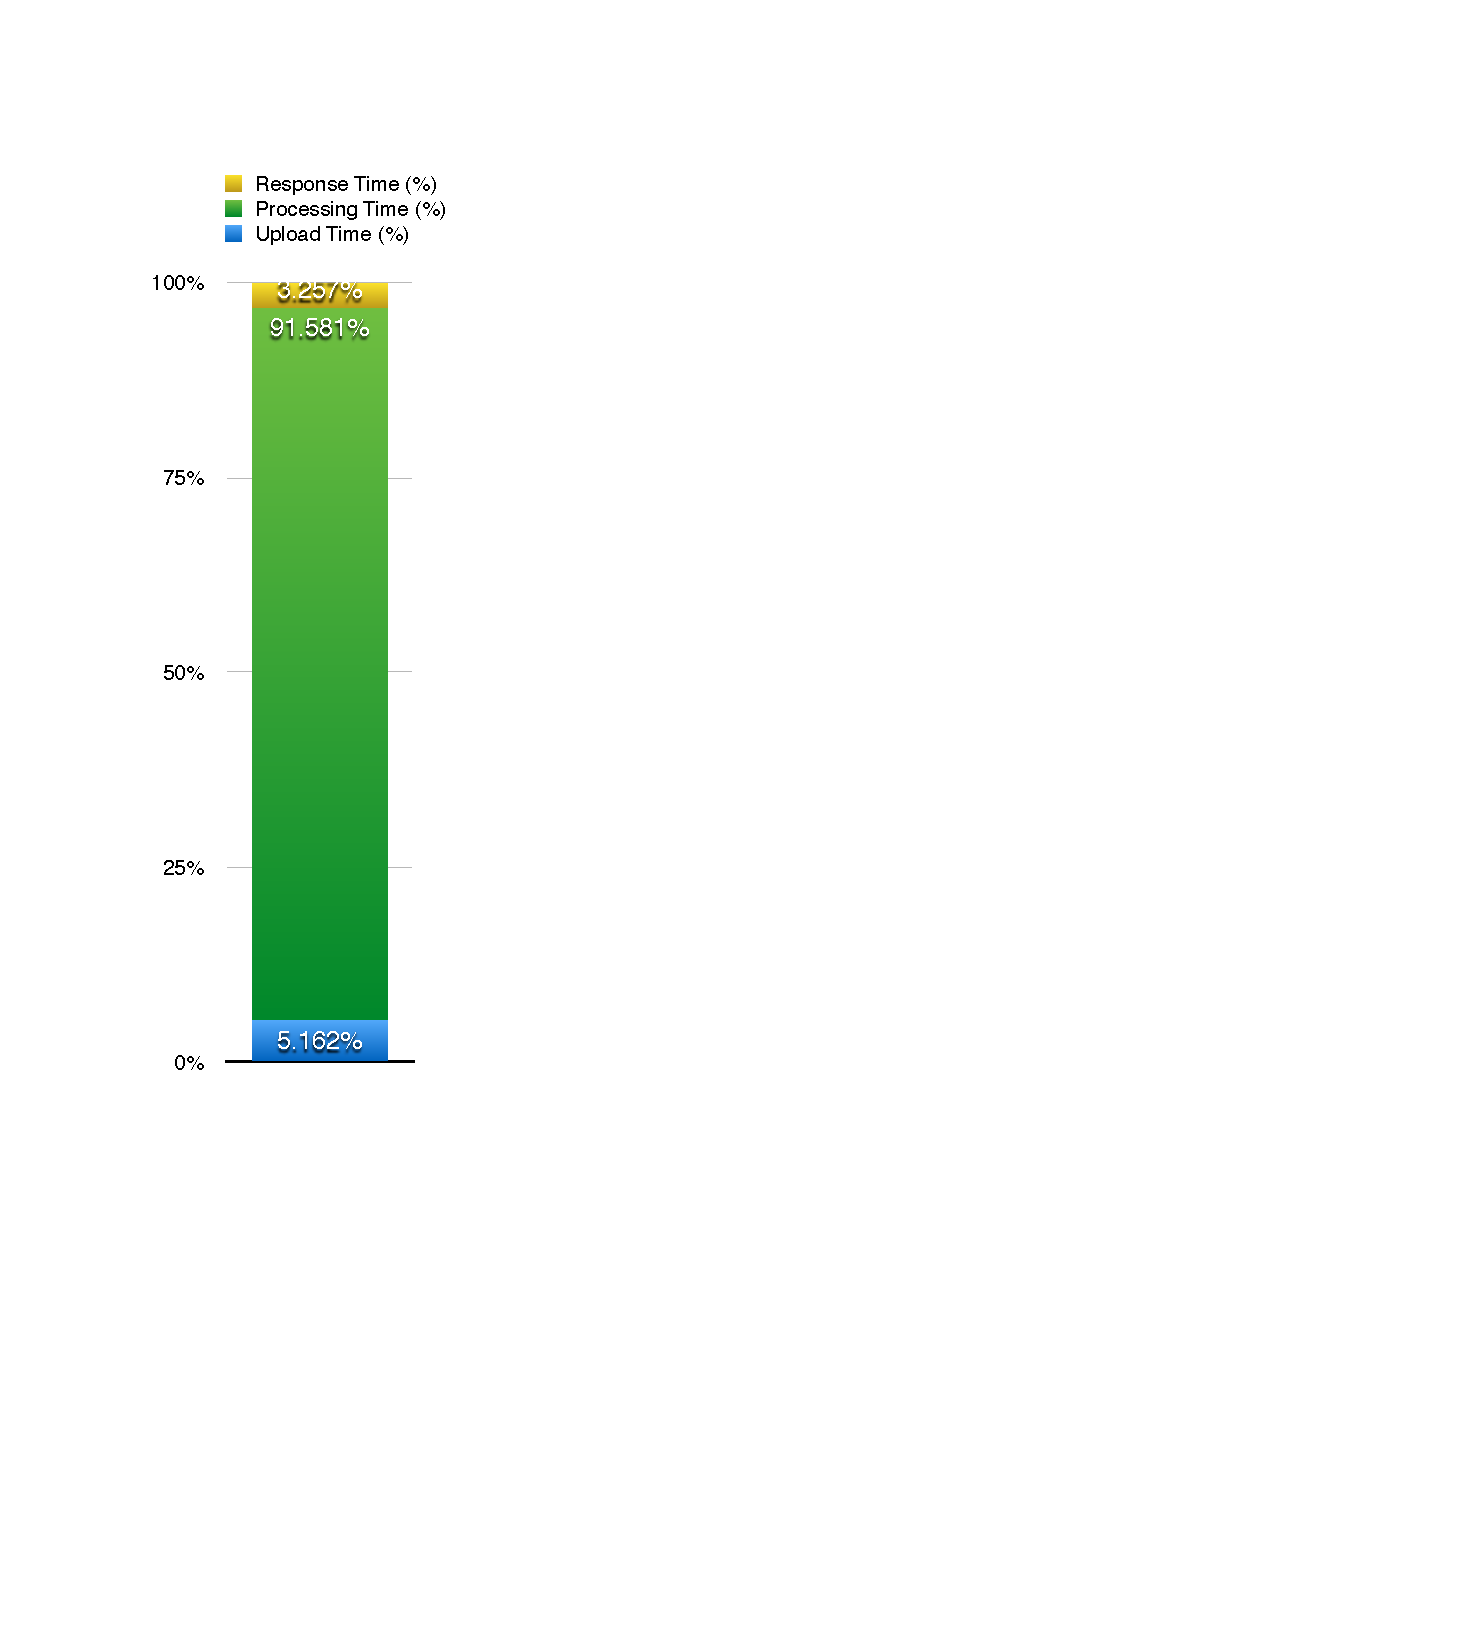
\includegraphics[width=.4\linewidth]{./images/ecspec_cloud_breakdown}
    \caption{Cloud-based approach: baseline\\Event Cycle latency breakdown.}
    \label{fig:ecspec_cloud}
  \end{subfigure}
  \caption{Baseline Event Cycle latency breakdown.}
  \label{fig:ecspec_breakdown}
\end{figure}

Figure~\ref{fig:ecspec_breakdown} presents the event latency breakdown for the current experiment.
Comparing the latency breakdown for the fog-based approach, presented in Figure~\ref{fig:ecspec_local},
with the cloud-based approach, presented in Figure~\ref{fig:ecspec_cloud}, it is possible to observe
that the value of the \textit{Upload Latency} and \textit{Response Latency} metrics for the cloud-approach
- close to 9$\%$ of the \textit{Event Latency} - is considerable higher when compared with the fog-approach,
where those values represent less then 0.5$\%$ of the \textit{Event Latency} metric. Is important to
point that the behavior for the \textit{Upload Latency} and \textit{Response Latency} metrics are
different for both approaches, in the fog-based approach the value of the \textit{Upload Latency}
metric is almost 50$\%$ higher then the \textit{Response Latency} metric, while in the cloud-based
approach those metrics presents the opposite behavior.\\

% % ECSpec local breakdown table
\begin{table}[ht!]
  \begin{tabular}{|c|c|c|c|c|}
  \hline
  ~                & Upload Time & Processing Time & Response Time & Event Latency \\ \hline
  Average Time (s) & 0.006       & 7.525           & 0.011         & 7.542         \\ \hline
  \end{tabular}
  \caption{Fog-based approach: baseline Event Cycle latency time.}
  \label{table:ecspec_local}
\end{table}

% % ECSpec cloud breakdown table
\begin{table}[ht!]
  \begin{tabular}{|c|c|c|c|c|}
  \hline
  ~                & Upload Time & Processing Time & Response Time & Event Latency \\ \hline
  Average Time (s) & 0.310       & 7.763           & 0.228         &  8.301        \\ \hline
  \end{tabular}
  \caption{Cloud-based approach: baseline Event Cycle latency time.}
  \label{table:ecspec_cloud}
\end{table}

Table~\ref{table:ecspec_local} and Table~\ref{table:ecspec_cloud} presents the latency values for the
current experiment. The metric values for the fog-based approach were obtained through the average
of 11 events that were generated during the experiment, while the values for the cloud-based were
obtained through the average of 9 events. Comparing the latency values for both approaches,
immediately is possible to observe that there is a huge difference between the values of the
\textit{Upload Latency} and \textit{Response Latency} metrics between both approaches. That
difference reflects in the value of the \textit{Event Latency} metric, where the fog-based approach
is almost 1s faster then the cloud-based approach.

\subparagraph{Half-Period Event Cycle}
\label{subp:eval_exp_latency_ecspec_fast}
In this scenario, we define the \textit{Half-period ECspec} to configure the \gls{ALE} module.
The configuration parameters are described in Table~\ref{table:ecspec_fast}.

% Half-period ECspec parameters
\begin{table}[ht!]
  \begin{tabular}{|c|c|}
    \hline
    Period & Duration \\ \hline
    5s    & 4.75s     \\ \hline
  \end{tabular}
  \caption{Half-period ECspec parameters.}
  \label{table:ecspec_fast}
\end{table}

\begin{figure}[ht!]
  \centering
  % ECSpec Fast local breakdown figure
  \begin{subfigure}{.5\textwidth}
    \centering
    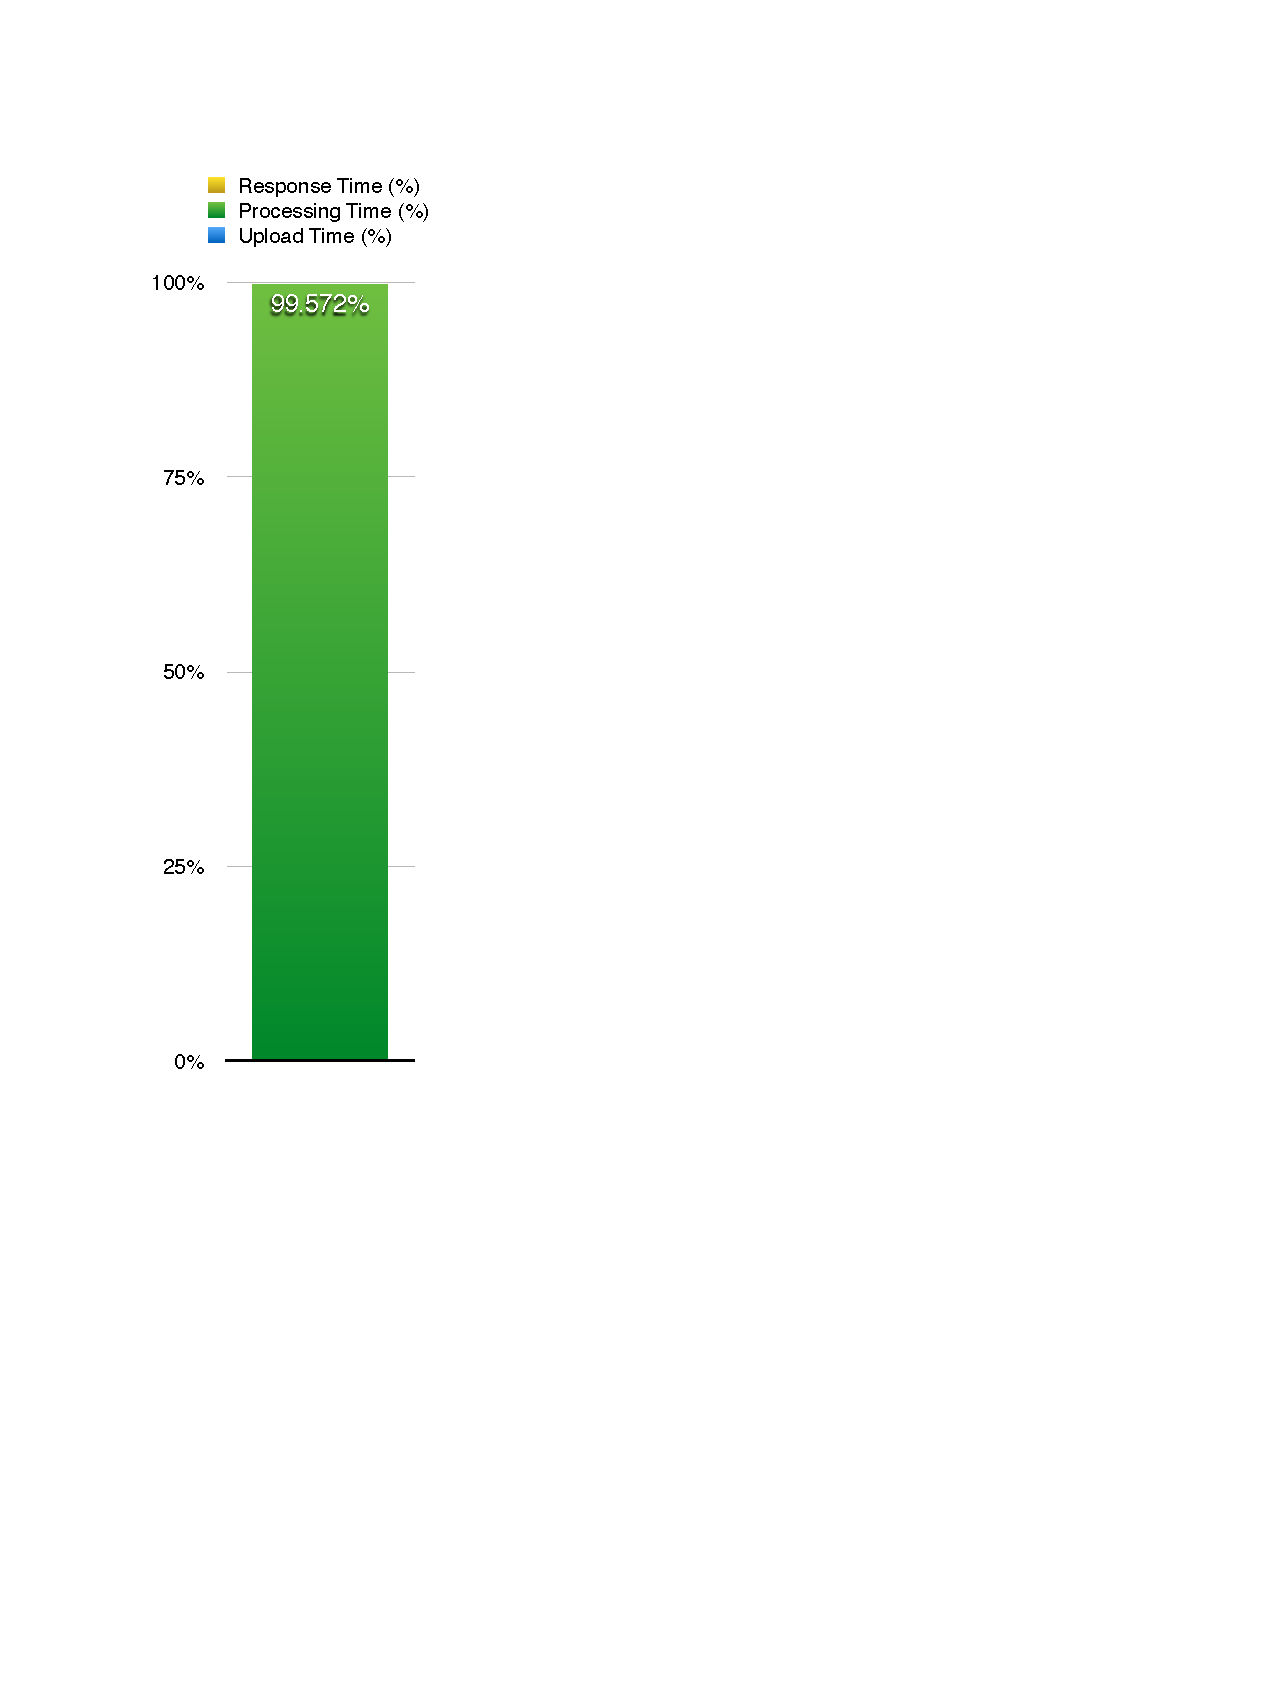
\includegraphics[width=.4\linewidth]{./images/ecspec_fast_local_breakdown}
    \caption{Fog-based approach: half-period Event Cycle\\ latency breakdown.}
    \label{fig:ecspec_fast_local}
  \end{subfigure}%
  % ECSpec fast cloud breakdown figure
  \begin{subfigure}{.5\textwidth}
    \centering
    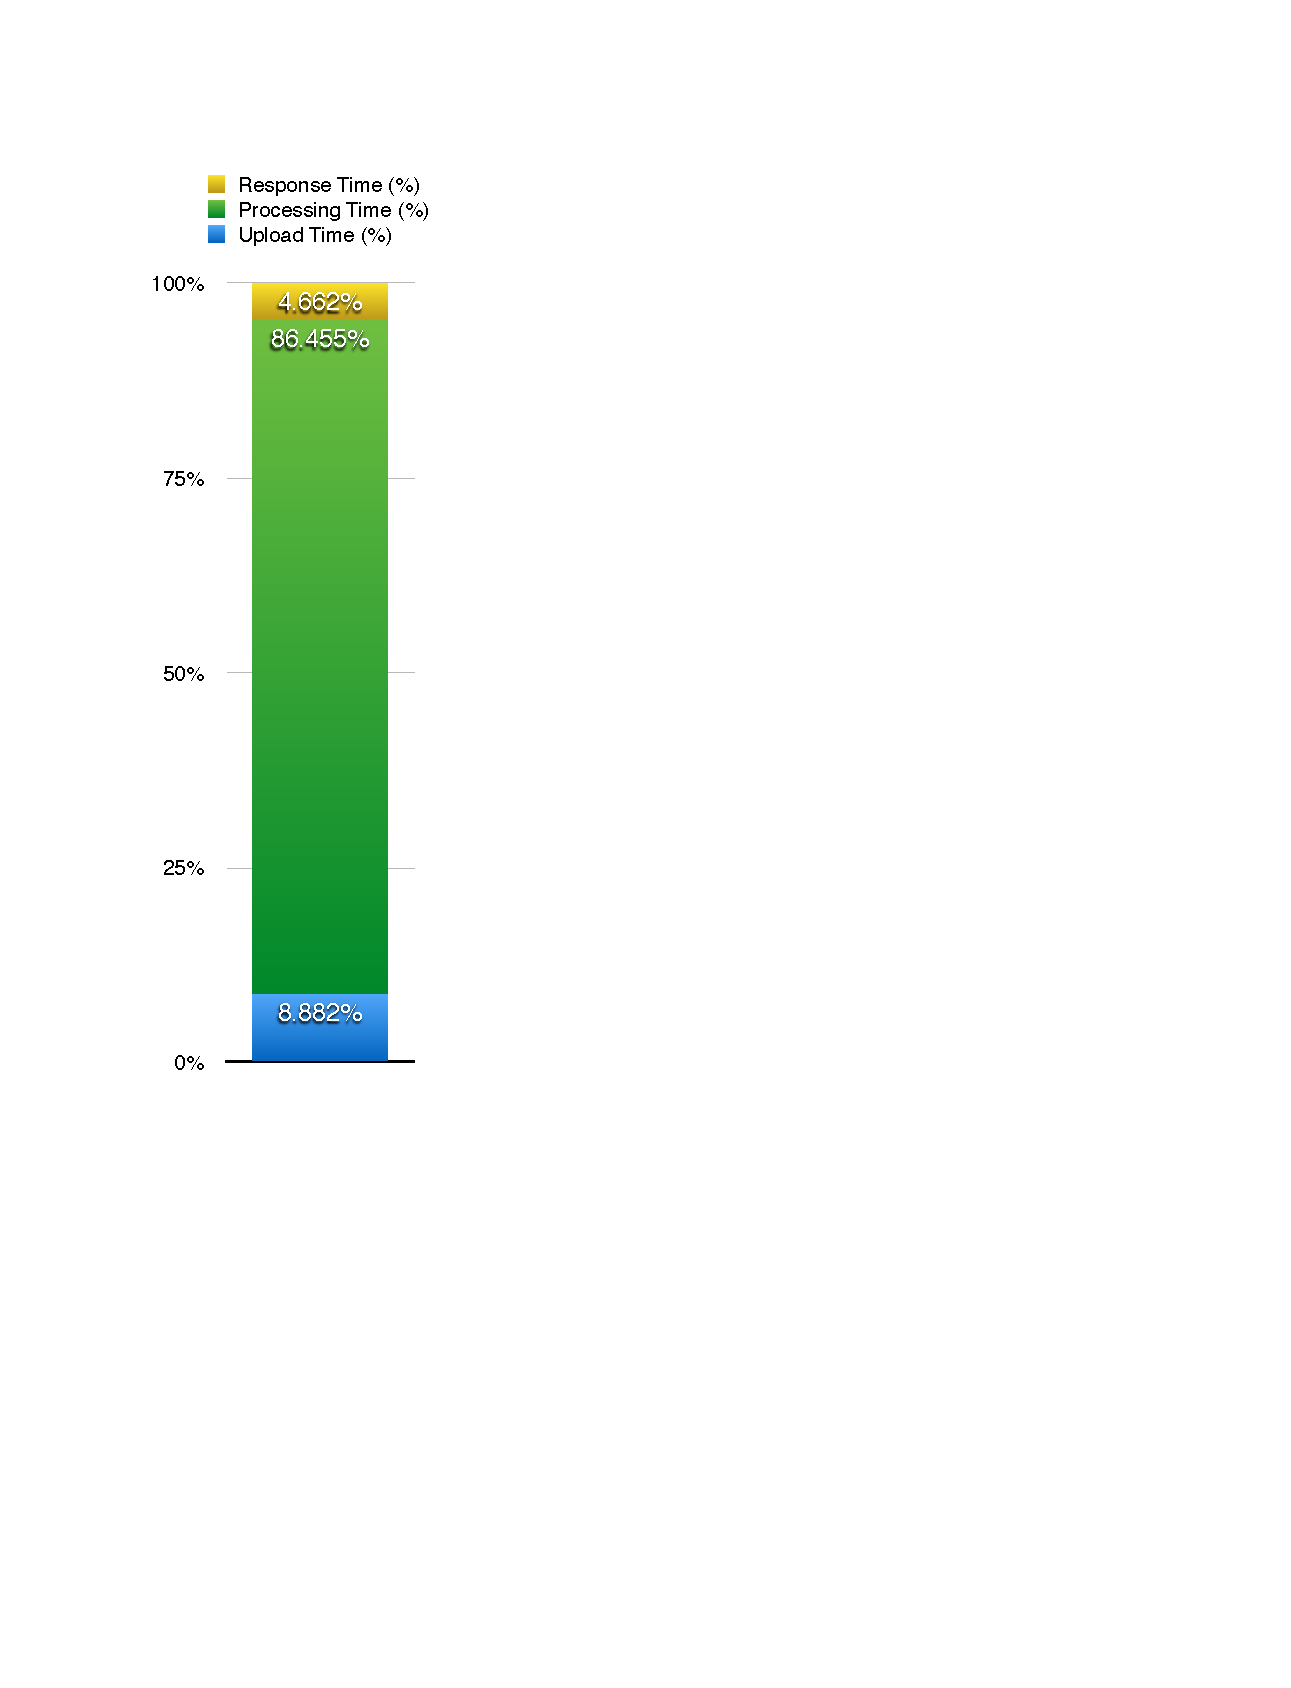
\includegraphics[width=.4\linewidth]{./images/ecspec_fast_cloud_breakdown}
    \caption{Cloud-based approach: half-period Event Cycle\\ latency breakdown.}
    \label{fig:ecspec_fast_cloud}
  \end{subfigure}
  \caption{Half-period Event Cycle latency breakdown.}
  \label{fig:ecspec_fast_breakdown}
\end{figure}

Figure~\ref{fig:ecspec_fast_breakdown} presents the event latency breakdown for the current experiment.
Comparing the latency breakdown for the fog-based approach, presented in Figure~\ref{fig:ecspec_fast_local},
with the cloud-based approach, presented in Figure~\ref{fig:ecspec_fast_cloud}, as in the previous experiment
it is possible to observe that the values of the \textit{Upload Latency} and \textit{Response Latency}
metrics for the cloud-approach are higher - close to 14$\%$ of the \textit{Event Latency} metric - to
the obtained in the \textit{Baseline} experiment, while the values obtained for the fog-approach
- close to 0.5$\%$ - maintained similar values. Regarding the behavior for those metrics, compared
with the \textit{Baseline} experiment, the behavior pattern observed in the previous experiment
was maintained.

% % ECSpec fast local breakdown table
\begin{table}[ht!]
  \begin{tabular}{|c|c|c|c|c|}
  \hline
  ~                & Upload Time & Processing Time & Response Time & Event Latency \\ \hline
  Average Time (s) & 0.006       & 4.216           & 0.010         & 4.232         \\ \hline
  \end{tabular}
  \caption{Fog-based approach: half-period Event Cycle latency time.}
  \label{table:ecspec_fast_local}
\end{table}

% % ECSpec fast cloud breakdown table
\begin{table}[ht!]
  \begin{tabular}{|c|c|c|c|c|}
  \hline
  ~                & Upload Time & Processing Time & Response Time & Event Latency \\ \hline
  Average Time (s) & 0.313       & 3.578           &  0.177        & 4.068         \\ \hline
  \end{tabular}
  \caption{Cloud-based approach: half-period Event Cycle latency time.}
  \label{table:ecspec_fast_cloud}
\end{table}

Table~\ref{table:ecspec_fast_local} and Table~\ref{table:ecspec_fast_cloud} present the latency values for the
current experiment. The metric values for the fog-based approach were obtained through the average
of 20 events that were generated during the experiment, while the values for the cloud-based were
obtained through the average of 23 events. As in the \textit{Baseline} experiment, the latency values
of the \textit{Upload Latency} and \textit{Response Latency} metrics presents a significant difference
between both approaches, where the values for the cloud-based approach continues to be higher.
However, in this experiment the fog-based approach present higher values for the \textit{Event Latency}
metric. Comparing the values presented in Table~\ref{table:ecspec_fast_local} and Table~\ref{table:ecspec_fast_cloud},
is possible to observe that the cause for that was the result tof he \textit{Processing Time}
metric, where the fog-based approach presented a better than the cloud-based approach.

% Evaluation Analysis
\section{Results Analysis and Discussion}
\label{sec:eval_analysis}
Based on the results obtained and in the requirements of application domains, it is possible to specify
which is the most adequate approach to deploy a smart place application that relies on \gls{RFID}
technology and in the Fosstrak middleware.

% Data scalability
\subparagraph{Data Scalability.}
\label{subp:eval_results_data}
Regarding the data scalability for the Fosstrak middleware, is possible to conclude that the metrics
of \textit{CPU Utilization} and \textit{Network In} increase as the threads and requests are growing.
These results are concise with the ones obtained by Gomes et al. \cite{gomes2014future}, which
proposes a new \gls{IoT} infrastructure for \gls{EPC}Global middleware. Moreover, in the experiments
performed Gomes detected that when the \textit{CPU Utilization} crosses the value of 95$\%$, the
outbound traffic started to decrease. After an analyzing the stored data, they conclude that the
\gls{CPU} exhaustion caused by the \gls{EPCIS} affected the performance of \gls{ALE} module,
resulting in a delay of data storage in the \gls{EPCIS} repository, which explains the observed
behavior.

% Latency Interaction
\subparagraph{Latency Interaction.}
\label{subp:eval_results_latency}
Regarding the latency interaction, it is clear that the fog-approach presented a better performance
than the cloud-based approach. However, there is a clear trade-off when choosing one of the proposed
approaches. In one side, the fog-based approach guarantees a better overall performance for the smart
place when compared with the cloud-based approach.\\

However, it is important to point that there some aspects that can improve the overall performance
of the cloud-based approach. For instance, the network connection is a possible bottleneck for the
performance of such approach. We believe that if the experiments were conducted through a faster
network connection - e.g. a Fiber-optic connection - the overall performance of the cloud-approach
will be better, but not as the fog-based approach.\\

In the other side, the fog-based approach requires an infrastructure burden that a cloud-based approach
is able to suppress. This is an important aspect to take in consideration when choosing one of the
approaches, since that a fog-based approach requires a large investment in infrastructure and the
performance gain offered by such approach could not be so substantial when compared with a cloud-based
approach.\\

\subparagraph{Fog or Cloud?}
\label{subp:eval_conclusion}
The obtained results shows that a fog-based approach offers better performance to deploy a smart
warehouse application based in \gls{RFID} technology that requires low latency interaction.
But it will be this approach the best choice for all application domains?\\

Table \ref{table:smart_places_requirements} presents the requirements of \gls{IoT} applications
for several domains. For instance, for application domains with a small network size, low network
bandwidth requirements, low scalability and does not require low latency interaction - such as Smart
Home/Office and Smart Retail scenarios - a cloud-based approach is suitable, but probably the more adequate
solution it will be to provisioning the infrastructure in local, since that in most cases a local
server is able to host such applications.\\

For domains with a medium/large network size and network bandwidth requirements, that does not require
a low latency interaction but presents high scalability - such as Smart Agriculture and Smart Water
scenarios - a cloud-based approach is the most reasonable choice. Finally, for domains with a
medium/large network size and network bandwidth requirements, that requires low latency interaction
and presents high scalability - such as Smart Cities and Smart Transportation scenarios - the
fog-based approach is the best solution.
